\begin{vd}

\begin{figure}[h]
    \centering
    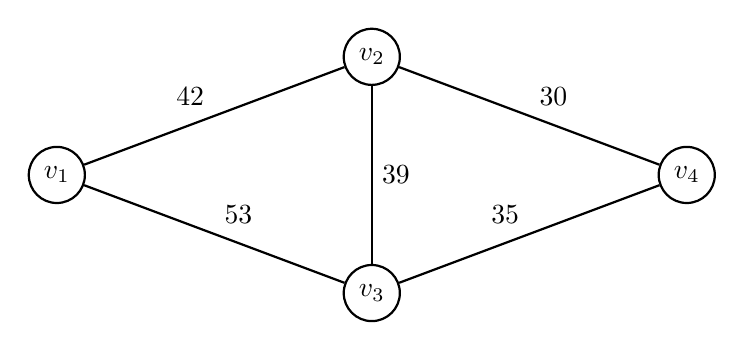
\begin{tikzpicture}[thick, main/.style = {draw, circle}, dis/.style = {}] 
        % Manual positions
        \node[main] (1) at (-4, 0) {$v_1$};
        \node[main] (2) at (0, 1.5) {$v_2$};
        \node[main] (3) at (0, -1.5) {$v_3$}; 
        \node[main] (4) at (4, 0) {$v_4$};  % symmetric middle right
        
        % Edges with weights
        \draw[-] (1) -- node[above left] {$42$} (2);
        \draw[-] (1) -- node[above right] {$53$} (3);
        \draw[-] (2) -- node[right] {$39$} (3);
        \draw[-] (2) -- node[above right] {$30$} (4);
        \draw[-] (3) -- node[above left] {$35$} (4);
    \end{tikzpicture} 
    \caption{Hình 2.1}
\end{figure}

\begin{equation*}
    D =
    \begin{Vmatrix}
        0 & 42 & 53 & 72 \\
        42 & 0 & 39 & 30 \\
        53 & 39 & 0 & 35 \\
        72 & 30 & 35 & 0
    \end{Vmatrix}.
\end{equation*}


\begin{figure}[h!]
    \centering
    \begin{tikzpicture}[scale=0.9]
    \begin{axis}[
        width=15cm,
        height=10cm,
        xlabel={$x$},
        ylabel={$F_j(x)$},
        legend pos=south east,
        axis lines=left,
        clip=true,
        xmin=0, xmax=42,
        ymin=20, ymax=75,
        enlarge y limits={abs=5},
    ]

        % f1(x): thin first (not in legend)
    \addplot[
        domain=0:9.5,
        samples=100,
        line width=1.5pt,
        orange,
        forget plot
    ] {x + 53};

    % f1(x): thick after (this one goes in legend)
    \addplot[
        domain=9.5:14,
        samples=100,
        line width=3pt,
        orange
    ] {x + 53};
    \addlegendentry{$f_1(x)$ của $d(v_3,x)$}


    % f2(x) for v3
    \addplot[
        domain=14:42,
        samples=100,
        line width=3pt,
        blue
    ] {42 - x + 39};
    \addlegendentry{$f_2(x)$ của $d(v_3,x)$}


    % f2(x) for v4: thick first (in legend)
    \addplot[
        domain=0:9.5,
        samples=100,
        line width=3pt,
        red
    ] {42 - x + 30};
    \addlegendentry{$f_2(x)$ của $d(v_4,x)$}

    % f2(x): thin tail (not in legend)
    \addplot[
        domain=9.5:42,
        samples=100,
        line width=1.5pt,
        red,
        forget plot
    ] {42 - x + 30};

    % Intersection point
    \addplot[
        only marks,
        mark=*,
        mark size=3pt,
        black
    ] coordinates {(14, 67)};

    % Node label
    \node at (axis cs:14,67) [xshift=0pt, yshift=15pt] {$(14,\ 67)$};
    
    % Intersection point
    \addplot[
        only marks,
        mark=*,
        mark size=3pt,
        black
    ] coordinates {(0, 72)};

    % Node label
    \node at (axis cs:0,72) [xshift=25pt, yshift=10pt] {$(0,\ 72)$};
    
    % Intersection point
    \addplot[
        only marks,
        mark=*,
        mark size=3pt,
        black
    ] coordinates {(9.5, 62.5)};

    % Node label
    \node at (axis cs:9.5,62.5) [xshift=0pt, yshift=-25pt] {$(9.5,\ 62.5)$};

    \end{axis}
    \end{tikzpicture}
    \caption{$B_1$}
\end{figure}

\begin{figure}[h!]
    \centering
    \begin{tikzpicture}[scale=0.9]
    \begin{axis}[
        width=15cm,
        height=10cm,
        xlabel={$x$},
        ylabel={$F_j(x)$},
        legend pos=south east,
        axis lines=left,
        clip=true,
        xmin=0, xmax=39,
        ymin=30, ymax=75,
        enlarge y limits={abs=5},
    ]

    \addplot[
        domain=0:25,
        samples=100,
        line width=3pt,
        orange
    ] {x + 42};
    \addlegendentry{$f_1(x)$ của $d(v_1,x)$}

    \addplot[
        domain=25:42,
        samples=100,
        line width=3pt,
        blue
    ] {-x + 92};
    \addlegendentry{$f_2(x)$ của $d(v_1,x)$}
    
    \addplot[
        domain=0:22,
        samples=100,
        line width=1.5pt,
        brown
    ] {x + 30};
    \addlegendentry{$f_1(x)$ của $d(v_4,x)$}
    
    \addplot[
        domain=22:42,
        samples=100,
        line width=1.5pt,
        red
    ] {39 - x + 35};
    \addlegendentry{$f_2(x)$ của $d(v_4,x)$}

    \addplot[
        only marks,
        mark=*,
        mark size=3pt,
        black
    ] coordinates {(25, 67)};

    \node at (axis cs:25,67) [xshift=0pt, yshift=15pt] {$(25,\ 67)$};
    
    \addplot[
        only marks,
        mark=*,
        mark size=3pt,
        black
    ] coordinates {(22, 52)};

    \node at (axis cs:22,52) [xshift=0pt, yshift=15pt] {$(22,\ 52)$};

    \end{axis}
    \end{tikzpicture}
    \caption{$B_2$}
\end{figure}

\begin{figure}[h!]
    \centering
    \begin{tikzpicture}[scale=0.9]
    \begin{axis}[
        width=15cm,
        height=10cm,
        xlabel={$x$},
        ylabel={$F_j(x)$},
        legend pos=south east,
        axis lines=left,
        clip=true,
        xmin=0, xmax=53,
        ymin=30, ymax=82,
        enlarge y limits={abs=5},
    ]

    \addplot[
        domain=23:25,
        samples=100,
        line width=3pt,
        orange
    ] {x + 42};
    \addplot[
        domain=0:23,
        samples=100,
        line width=1.5pt,
        orange,
        forget plot
    ] {x + 42};
    \addlegendentry{$f_1(x)$ của $d(v_2,x)$}

    \addplot[
        domain=25:53,
        samples=100,
        line width=3pt,
        blue
    ] {53 - x + 39};
    \addlegendentry{$f_2(x)$ của $d(v_2,x)$}
    
    \addplot[
        domain=0:8,
        samples=100,
        line width=3pt,
        red
    ] {x + 72};
    \addlegendentry{$f_1(x)$ của $d(v_4,x)$}
    
    \addplot[
        domain=8:23,
        samples=100,
        line width=3pt,
        brown
    ] {53 - x + 35};
    \addplot[
        domain=23:53,
        samples=100,
        line width=1.5pt,
        brown,
        forget plot
    ] {53 - x + 35};
    \addlegendentry{$f_2(x)$ của $d(v_4,x)$}

    \addplot[
        only marks,
        mark=*,
        mark size=3pt,
        black
    ] coordinates {(25, 67)};

    \node at (axis cs:25,67) [xshift=0pt, yshift=15pt] {$(25,\ 67)$};

    \addplot[
        only marks,
        mark=*,
        mark size=3pt,
        black
    ] coordinates {(8, 80)};

    \node at (axis cs:8,80) [xshift=0pt, yshift=15pt] {$(8,\ 80)$};
    
    \addplot[
        only marks,
        mark=*,
        mark size=3pt,
        black
    ] coordinates {(23, 65)};

    \node at (axis cs:23,65) [xshift=0pt, yshift=-25pt] {$(23,\ 65)$};
    \end{axis}
    \end{tikzpicture}
    \caption{$B_3$}
\end{figure}



\begin{figure}[h!]
    \centering
    \begin{tikzpicture}[scale=0.9]
    \begin{axis}[
        width=15cm,
        height=10cm,
        xlabel={$x$},
        ylabel={$F_j(x)$},
        legend pos=south east,
        axis lines=left,
        clip=true,
        xmin=0, xmax=35,
        ymin=30, ymax=82,
        enlarge y limits={abs=5},
    ]

    \addplot[
        domain=0:27,
        samples=100,
        line width=3pt,
        orange
    ] {x + 53};
    \addlegendentry{$f_1(x)$ của $d(v_1,x)$}

    \addplot[
        domain=27:35,
        samples=100,
        line width=3pt,
        blue
    ] {35 - x + 72};
    \addlegendentry{$f_2(x)$ của $d(v_1,x)$}
    

    \addplot[
        only marks,
        mark=*,
        mark size=3pt,
        black
    ] coordinates {(27, 80)};

    \node at (axis cs:27,80) [xshift=0pt, yshift=15pt] {$(27,\ 80)$};

    \end{axis}
    \end{tikzpicture}
    \caption{$B_4$}
\end{figure}


\begin{figure}[h!]
    \centering
    \begin{tikzpicture}[scale=0.9]
    \begin{axis}[
        width=15cm,
        height=10cm,
        xlabel={$x$},
        ylabel={$F_j(x)$},
        legend pos=south east,
        axis lines=left,
        clip=true,
        xmin=0, xmax=53,
        ymin=30, ymax=82,
        enlarge y limits={abs=5},
    ]

    \addplot[
        domain=23:25,
        samples=100,
        line width=3pt,
        orange
    ] {x + 42};
    \addplot[
        domain=0:23,
        samples=100,
        line width=1.5pt,
        orange,
        forget plot
    ] {x + 42};
    \addlegendentry{$f_1(x)$ của $d(v_2,x)$}

    \addplot[
        domain=25:53,
        samples=100,
        line width=3pt,
        blue
    ] {53 - x + 39};
    \addlegendentry{$f_2(x)$ của $d(v_2,x)$}
    
    \addplot[
        domain=0:8,
        samples=100,
        line width=3pt,
        red
    ] {x + 72};
    \addlegendentry{$f_1(x)$ của $d(v_4,x)$}
    
    \addplot[
        domain=8:23,
        samples=100,
        line width=3pt,
        brown
    ] {53 - x + 35};
    \addplot[
        domain=23:53,
        samples=100,
        line width=1.5pt,
        brown,
        forget plot
    ] {53 - x + 35};
    \addlegendentry{$f_2(x)$ của $d(v_4,x)$}

    \addplot[
        only marks,
        mark=*,
        mark size=3pt,
        black
    ] coordinates {(25, 67)};

    \node at (axis cs:25,67) [xshift=0pt, yshift=15pt] {$(25,\ 67)$};

    \addplot[
        only marks,
        mark=*,
        mark size=3pt,
        black
    ] coordinates {(8, 80)};

    \node at (axis cs:8,80) [xshift=0pt, yshift=15pt] {$(8,\ 80)$};
    
    \addplot[
        only marks,
        mark=*,
        mark size=3pt,
        black
    ] coordinates {(23, 65)};

    \node at (axis cs:23,65) [xshift=0pt, yshift=-25pt] {$(23,\ 65)$};
    \end{axis}
    \end{tikzpicture}
    \caption{$B_5$}
\end{figure}



\end{vd}